
\section{INTRODUCTION AND MOTIVATION}
% \section{Matrix formulation of the problem - 1D interferometer}
% 
% Here I intend to use convolution matrices properties to {\it qualitatively} study how ``pseudo-PSF'' vary as a
% function of source location. Here I limit myselves to a 1-dimensional
% interferometer (scalar only), so that
% Convolution matrices are Toeplitz-symetyric (see bellow). In a more
% general case, (along my intuition - but should be thought more
% carefully), convolution matrices should be block-Toeplitz (each
% block is a Toeplitz), while symetricity should still be true. 
% 
% \subsection{Remarks on the convolution and linear algebra}
% 
% In functional form the convolution theorem can be written as follows:
% 
% 
% \def\F{\mathcal{F}}
% \def\Fm{\bm{F}}
% \def\Gauss{\bm{\mathcal{G}}}
% \def\conv{\mathcal{*}}
% 
% \begin{alignat}{2}
% %\label{eq:Lin}
% %\F \left{ a.b\right}=&\F \left{ a\right}.\F \left{b\right}\\
% \F \left\{  a.b\right\}=& \F \left\{a\right\}\conv\F \left\{b\right\}
% \end{alignat}
% 
% Noting the convolution product is linear, we can reexpress the
% convolution product and associated theorem asing linear
% transformations:
% 
% \newcommand{\C}[1]{\bm{\mathcal{C}}_{#1}}
% \newcommand{\vv}[1]{\bm{#1}}
% \def\one{\bm{1}}
% 
% 
% \begin{alignat}{2}
% \label{eq:ConvTh}
% %\F \left{ a.b\right}=&\F \left{ a\right}.\F \left{b\right}\\
% \Fm \vv{A}\vv{b}=& \C{\vv{A}}\Fm \vv{b}
% \end{alignat}
% 
% \noindent where $\Fm$ is the Fourier operator of size 
% $n_{uv}\times n_{lm}$ ($\Fm$ is unitary $\Fm^H\Fm=\one$), $\vv{b}$ is
% a vector with size $n_{lm}$. The matrix $\vv{A}$ models the scalar
% multiplication of each point in $\vv{b}$, and is therefore diagonal of
% size $n_{lm}\times n_{lm}$, and $\C{\vv{A}}$ is the convolution matrix
% of size $n_{uv}\times n_{uv}$. There is a bijective relation
% 
% \begin{alignat}{2}
% \label{eq:ConvTh}
% %\F \left{ a.b\right}=&\F \left{ a\right}.\F \left{b\right}\\
% \vv{A} \longleftrightarrow \C{\vv{A}}
% \end{alignat}
%  
% \noindent in the sense that a scalar multiplucation defines a convolution
% function and conversely. The matrices $\vv{A}$ and $\C{\vv{A}}$ always
% have the following properties:
% 
% \begin{itemize}
%   \item $\vv{A}$ is diagonal
% 
%    \item In the 1D case
% \begin{itemize}
%   \item $\C{\vv{A}}$ is Toeplitz
%   \item In addition, for radiointerferometry, because the uv plane is symetric, $\C{\vv{A}}$ is symetric
% \end{itemize}
% 
% \end{itemize}
% 
% The matrix $\C{\vv{A}}$ being Toeplitz, each row $\left[ \C{\vv{A}}
%   \right]_l$ with sky coordinate $l$ can be built using a
% rolling operator $\Delta_l$ that shifts the first row (the PSF at the field
% center for example) to location of row $l$:
% 
% \begin{alignat}{2}
% \label{eq:ConvTh}
% %\F \left{ a.b\right}=&\F \left{ a\right}.\F \left{b\right}\\
% \left[ \C{\vv{A}} \right]_l =& \Delta_l \left\{ \left[ \C{\vv{A}} \right]_0 \right\}
% and&\\
% \left[ \C{\vv{A}} \right]_0 =& \Fm^H \ \text{diag}(\vv{A})
% \end{alignat}
% 
% The rolling operator is essentially just a reindexing, and has the
% following properties:
% 
% \begin{alignat}{2}
% \label{eq:PropsDelta0}
% %\F \left{ a.b\right}=&\F \left{ a\right}.\F \left{b\right}\\
% \Delta_l \left\{ a\vv{x} \right\} =&  a \Delta_l \left\{\vv{x} \right\} \\
% \label{eq:PropsDelta1}
% \Delta_l \left\{ \sum_i \vv{x}_i \right\} =& \sum_i \Delta_l \left\{ \vv{x}_i \right\} 
% \end{alignat}
% 
% \newcommand{\roll}[1]{\Delta_l \left\{#1\right\}}
% 
% 
% \subsection{PSF behaviour}
% 
% If $\vv{X}$ is the true sky, then the dirty image $\vv{X}^D_{ij}$ of
% baseline $(ij)$ can be written as:
% 
% \begin{alignat}{2}
% \vv{x}^D_{ij} =& \Fm^H \vv{S}_{c,ij}  \C{\vv{T}} \vv{S}_{\square,ij} \Fm \vv{A} \vv{x}
% \end{alignat}
% 
% \noindent where $\vv{A}_{ij}$ models the DDE effets and is an
% $n_{pix}\times n_{pix}$ diagonal matrix (taking polarisation into
% account it is an
% $4n_{pix}\times 4n_{pix}$ block diagonal matrix), $\vv{T}$ is the tapering/averaging function, 
% $\vv{S}_{\square}$ samples the region over which the
% tapering/averaging is made, and $\vv{S}_{c,ij}$ selects the central point
% of the averaged/tapered visibility set. Using Eq. \ref{eq:ConvTh}, we have:
% 
% \begin{alignat}{2}
% \vv{x}^D_{ij} =&\ \C{\vv{S}_{c,ij}}  \vv{T} \C{\vv{S}_{\square,ij}}  \Fm^H \Fm \vv{A}_{ij} \vv{x}\\ 
%  =&\  \C{\vv{S}_{c,ij}}  \vv{T} \C{\vv{S}_{\square,ij}}  \vv{A}_{ij}  \vv{x}\\ 
% \label{eq:approx}
%  \sim&\  \C{\vv{S}_{c,ij}}  \vv{T}    \vv{A}_{ij} \vv{x}
% \end{alignat}
% 
% \noindent where Eq. \ref{eq:approx} is true when the support of the
% function $T$ is smaller than the sampling domain of
% $\vv{S}_{\square}$. 
% 
% Averaged over all baselines, the dirty image becomes:
% 
% \begin{alignat}{2}
% \label{eq:PPSF}
% \vv{x}^D =&\bm{\mathcal{C}}_{STA} \vv{x}\\
% \text{with }\bm{\mathcal{C}}_{STA}=&\sum_{ij}  \C{\vv{S}_{c,ij}}  \vv{T}    \vv{A}_{ij}
% \end{alignat}
% 
% 
% 
% \subsection{Deriving the Pseudo-PSF}
% 
% \subsubsection{PSF and Pseudo-PSF}
% 
% {\bf We can already see that $\C{\vv{S}_{c,ij}}
%   \vv{T}    \vv{A}_{ij}$ in Eq. \ref{eq:approx} is NOT Toeplitz anymore
%   because each colunm is multiplied by a different value (DDE
%   muliplied by the tapering function). The dirty sky is therefore not
%   anymore the convolution of the true sky by the psf} {\it ie} the PSF
% varies accross the field of view.
% 
% \subsubsection{Slow way}
% 
% Calculate the psf estimating $\mathcal{C}$ from direct
% calculation. Eventually at discrete locations on a grid.
% 
% 
% \subsubsection{Quickly deriving the Pseudo-PSF}
% 
% This is tricky part. The problem amount to finding any column $l$ of
% $\bm{\mathcal{C}}$ on demand. For notation convenience, we merge
% $\vv{T}$ and $\vv{A}_{ij}$ together in $\vv{A}_{ij}$. Operator
% $\left[\vec{M}\right]_l$ extracts column $l$ from matrix $\vec{M}$,
% and using Eq. \ref{eq:PropsDelta0}, \ref{eq:PropsDelta1} and \ref{eq:PPSF}:
% 
% \begin{alignat}{2}
% \left[\bm{\mathcal{C}}\right]_l =&
%      \left[\sum_{ij}  \C{\vv{S}_{c,ij}}  \vv{A}_{ij}\right]_l\\
% =& \sum_{ij} a^l_{ij} \left[\C{\vv{S}_{c,ij}}\right]_l \\
% &\ \ \ \text{with } a^l_{ij}=\vv{A}_{ij}(l)\\
% =& \sum_{ij} \roll{a^l_{ij} \left[\C{\vv{S}_{c,ij}}\right]_0} \\
% =& \sum_{ij} \roll{\Fm^H a^l_{ij}\ \text{diag}\left(\vv{S}_{c,ij}\right) }
% \end{alignat}
% 
% If we now assume that at any given location $l$, the scalar $a^l_{ij}$
% can be described by a smooth {\it function} of the uv coordinates
% ($(ij)$-indices), then we can write:
% 
% \begin{alignat}{2}
% \left[\bm{\mathcal{C}}\right]_l =
% & \sum_{ij} \roll{ \Fm^H \vv{A}^l\ \text{diag}\left(\vv{S}_{c,ij}\right) }\\
% =& \sum_{ij} \roll{\C{\vv{A}^l}\ \Fm^H \text{diag}\left(\vv{S}_{c,ij}\right) }\\
% =& \sum_{ij} \roll{\C{\vv{A}^l}\ \left[\C{\vv{S}_{c,ij}}\right]_0 }\\
% =& \roll{\C{\vv{A}^l}\ \sum_{ij} \left[\C{\vv{S}_{c,ij}}\right]_0 }\\
% =& \roll{\C{\vv{A}^l}\ \left[\C{\vv{S}_{c}}\right]_0 }\\
% \end{alignat}
% 
% The approximate observed Pseudo-PSF is the convolution of the PSF at
% the phase center ($\left[\C{\vv{S}_{c}}\right]_0$) and the fourier transform of the uv-dependent tapering function at given
% lm ($\C{\vv{A}^l}$).
% 
% In other words, to compute the PSF at a given location $(lm)$:
% 
% \begin{itemize}
%   \item Find $\vv{A}$:
%     \begin{itemize}
%     \item Compute weight $w_{ij}$ for each baseline $(ij)$
%     \item Fit the uv-dependent weight by (for example), a Gaussian function $w_{ij}\sim w(u,v)=\Gauss\left(u,v\right)$ 
%     \end{itemize}
%   \item Compute the $PSF_{lm}$ at $(lm)$ from the PSF at the phase center $PSF_0$ as $PSF_{lm}=\mathcal{F}^{-1}\left(w\right)\conv PSF_0$
% \end{itemize}
% For example if the long baselines are more tapered, they are
% "attenuated". The effective PSF on the edge of the field will get
% larger by the convolution...
% Something like that...
% %\section{Numerical Experiments}
% %We demonstrate the computational complexity of the quick, the slow derived PSF as a function of sky coordinates and 
%perform a direct numerical results.
\section{PROBLEM STATEMENT and PSF SLOW DERIVATION}
We demonstrate the computational complexity of the quick, the slow derived PSF as a function of sky coordinates and 
perform a direct numerical results.
\subsection{interferometric visibility}
It is worth noting that in the Radio Astronomy community the cross-correlator output of two elements interferometer
in response to a source with spectral brightness distribution $I_{\nu}(\mathbf{s})$ as a function of the pointing direction $\mathbf{s}$ 
is the visibility function defined in Eq.\ref{eq:1} and obtained by integrating
over the solid angle $d\Omega$ \citep{thompson2008interferometry,taylor1999synthesis}
\begin{alignat}{2}
V_{}(\mathbf{b}) =& \int_{\Omega}I_{\nu}(\mathbf{s})e^{-2\pi i \mathbf{b}\mathbf{s}}d\Omega, \label{eq:1}
\end{alignat}
where $\mathbf{b}=\mathbf{b}(t,\nu)=(u_{t\nu}, v_{t\nu}, w_{t\nu})$  is the so-called "\textit{baseline vector}" in wavelength
and with modulus the distance between the two elements
interferometer. The measurement in Eq.\ref{eq:1} is over the entire 
surface of the celestial sphere, practically the measurement is generally taken over a finite surface area of 
the celestial sphere due to the finite nature of the tracking source and other effects. Furthermore, the result is
averaged over finite time/frequency bins. Suppose $\Delta t$ centered at $t_0$ and $\Delta \nu$ centered at $\nu_0$ the 
time and frequency sampling intervals respectively. 
Assuming that $\Delta t$ and  $\Delta \nu$ are small  enough so that $I_{\nu}(\mathbf{s})$
remains constant while the complex phase, $-2\pi i \mathbf{b}\mathbf{s}$ varies linearly.   Eq. \ref{eq:1} becomes:
\begin{alignat}{2}
V_{}(t_0,\nu_0) =& \frac{1}{\Delta t \Delta \nu}\iint\limits_{\Delta t \Delta \nu}^{}\bigg[\int\limits_{\Omega}^{}I_{\nu}(\mathbf{s})e^{-2\pi i \mathbf{b}\mathbf{s}} d\Omega\bigg] dt d\nu. \label{eq:2}	    
\end{alignat}
However, performing the integration over a surface of size, $\Delta t \times \Delta \nu$ yields a nonzero value only in 
this surface area, which is recognized as integrating of a windowing function  $\Pi_{t_0,\nu_0}(t,\nu)$ of size $\Delta t \times \Delta \nu$.
Let $\mathbf{b}_0=\mathbf{b}(t_0,\nu_0)=(u_{t_0\nu_0}, v_{t_0\nu_0}, w_{t_0\nu_0})$ be the baseline vector at the centre
of the sampling intervals and $W_{t_0,\nu_0}(t,\nu)$ a weighting  sampling function. A generalized sampling kernel 
for a given $(u,v)$ track,
$W_{\mathbf{b}_0}(\mathbf{b})$  associated with the windowing function can be defined as
\begin{alignat}{2}
W_{\mathbf{b}_0}(\mathbf{b}) &=	\frac{\Pi_{t_0,\nu_0}(t,\nu)}{\Delta t \Delta \nu}W_{t_0,\nu_0}(t,\nu)\\
			      &=\frac{\Pi(\mathbf{b}-\mathbf{b}_0)}{\Delta u_{t\nu} \Delta v_{t\nu}}W(\mathbf{b}-\mathbf{b}_0).\label{eq:W}
\end{alignat}
% 
% 
% Let $W_{\mathbf{b}_0}(\mathbf{b})$ be the sampling kernel for a given $(u,v)$ bin where 
% the shorthand notation $W_{\mathbf{b}_0}(\mathbf{b})=\frac{W_{t_0,\nu_0}(t,\nu)}{\Delta t \Delta \nu}$ has been used. 
where, $\frac{dt d\nu}{du_{t\nu} dv_{t\nu}}=\frac{\Delta t \Delta \nu}{\Delta u_{t\nu} \Delta v_{t\nu}}$. Similary,  Eq.\ref{eq:2} can be written in terms 
of $\mathbf{b}_0$ and can thus be expressed as an integration over uv-bins.
We can write
\begin{alignat}{2}
V_{\mathbf{b}_0}(\mathbf{x})  =& \iint\limits_{u_{t\nu}v_{t\nu}}^{}W_{\mathbf{b}_0}(\mathbf{b})\bigg[\int\limits_{\Omega}^{}I_{\nu}(\mathbf{s})e^{-2\pi i \mathbf{b}\mathbf{s}}d\Omega \bigg]du_{t\nu} dv_{t\nu},  \label{eq:3}
\end{alignat}
% where the following shorthand notation has been used.
% \begin{alignat*}{2}
% \hspace{-1cm}\mathbf{b}_0=&\mathbf{b}(t_0,\nu_0)\\
% 			 =&(u_{t_0\nu_0}, v_{t_0\nu_0}, w_{t_0\nu_0}),\\
% \hspace{-1cm}W_{\mathbf{b}_0}(\mathbf{b})&=\frac{W_{t_0,\nu_0}(t,\nu)}{\Delta t \Delta \nu}.
% \end{alignat*}
%  Here, $\mathbf{b}_0$ is the baseline vector at centre
% of a sampling interval and the sampling kernel $W_{\mathbf{b}_0}(\mathbf{b})$ is defined as:
% of a sampling interval and the sampling kernel $W_{\mathbf{b}_0}(\mathbf{b})$ is defined as:
% \begin{alignat}{2}
% W_{\mathbf{b}_0}(\mathbf{b})&=\Pi(\mathbf{b}-\mathbf{b}_0)w(\mathbf{b}-\mathbf{b}_0),
% \end{alignat}
% where, $\Pi(\mathbf{b}-\mathbf{b}_0)$ is a windowing function and $w(\mathbf{b}-\mathbf{b}_0)$ a weighting kernel.\\
where, $\mathbf{x}=(u,v,w)$ the resulting average baseline vector.
As previously mentioned, we are interested in PSF response. Therefore, Eq.\ref{eq:3} is restricted to the
complex visibility measured by the two-element interferometer for a point source located towards the direction 
$\mathbf{s}$ with unit brightness. That said, $I_{\nu}(\mathbf{s})=\delta(\mathbf{b}_0)$ with $\delta$ the Dirac delta. 
It then follows that Eq\ref{eq:3} can be written as
\begin{alignat}{2}
V_{\mathbf{b}_0}(\mathbf{x})  =&\iint\limits_{u_{t\nu}v_{t\nu}}W_{\mathbf{b}_0}(\mathbf{b}) e^{-2\pi i (u_{t\nu}l+v_{t\nu}m+w_{t\nu}(n-1))}du_{t\nu}dv_{t\nu}. \label{eq:4}
\end{alignat} 
Note that Eq.\ref{eq:4} is obtained after a
delay correction of $\mathbf{b}\mathbf{s_0}$ is  applied to the signals from the antennas 
array to steer towards the direction $\mathbf{s}_0$ and $\mathbf{b}(\mathbf{s}-\mathbf{s_0})=u_{t\nu}l + v_{t\nu}m+w_{t\nu}(n-1)$ 
describes  the time difference between the two incoming signals. The three direction cosines $l,m$ and $n$ are components
of  $\mathbf{s}-\mathbf{s_0}$  in radians with $n=\sqrt{1-l^2-m^2}$.
For an extensive discussion, see \citep{thompson2008interferometry,taylor1999synthesis,leshem2000radio}.
Let  $G_{\mathbf{b}}(l,m)=e^{-2\pi i[w_{t\nu}(n-1)]}$ the fringe from the $w$-term. The $w$-term depends on the variation of
$u_{t\nu}$ and $v_{t\nu}$. In other words, $w_{t\nu}=(\gamma + \alpha  du_{t\nu} + \beta dv_{t\nu})$; $\gamma, \alpha,\beta$ are reals numbers.
In this paper, we consider the $w$-term in 
the general case where the array is coplanar ($w_{t\nu}=0$) or not ($w_{t\nu}\neq 0$) and/or when the array is
tracking a small field ($n \approx 1$) or a wide field ($n \ll 1$). The fringe from the $w$-term is separated; 
the measurement in Eq\ref{eq:4} becomes  a two dimensional 
Fourier transform. Making use of the convolution theorem which  
states that the Fourier transform of the product of two functions result in a convolution and vice-versa
\footnote{$http://mathworld.wolfram.com/ConvolutionTheorem.html$ $http://en.wikipedia.org/wiki/Convolution\_theorem$}, 
we have
\begin{alignat}{2}
V_{\mathbf{b}_0}(\mathbf{x})  =\widetilde{G}_{\mathbf{b}}(l,m)\circ &\iint\limits_{u_{t\nu}v_{t\nu}}W_{\mathbf{b}_0}(\mathbf{b}) e^{-2\pi i (u_{t\nu}l+v_{t\nu}m)}du_{t\nu}dv_{t\nu}. \label{eq:5}
\end{alignat} 
Also, $W_{\mathbf{b}_0}(\mathbf{b})$ is defined as a product of two functions (refer to Eq. \ref{eq:W}), making use
of the shifted Fourier transform properties and the convolution theorem, the following expansion is valid
\begin{alignat}{2}
V_{\mathbf{b}_0}(\mathbf{x}) =&\Bigg(\widetilde{G}_{\mathbf{b}}\circ\Big[C_{\mathbf{b}_0}\widetilde{\Pi}_{\mathbf{b}}\Big]
		    \circ &\Big[C_{\mathbf{b}_0}\widetilde{W}_{\mathbf{b}}\Big]\Bigg)(l,m)  \label{eq:6}
\end{alignat}
The symbols $\circ$ and  $\widetilde{}$ denote the convolution operator and the Fourier transform respectively.  The phase gradient, 
$C_{\mathbf{b}_0}(l,m)$  is defined as
\begin{alignat}{2}
C_{\mathbf{b}_0}(l,m) &=e^{-2\pi i (u_{t_0\nu_0}l+v_{t_0\nu_0}m)}
\end{alignat}
\subsubsection{Computational cost} 
\section{PSF QUICK DERIVATION}
In order to further optimize the slow derivation of the PSF described above to particularly reduce its computational
cost, we will need to understand the concept and theory of signal correlation in aperture synthesis.
% This expansion will be used to approximate the averaged or weighted averaged visibility
% $V_{}(\mathbf{b}_0)$.
If it is assumed that $\Pi(\mathbf{b})$ is the top-hat windowing function, then it can be demonstrated 
that its Fourier transform is (see Appendix A)
\begin{alignat}{2}
\widetilde{\Pi}(\mathbf{b})&=sinc\Big(\frac{-2\pi t\Delta \nu}{2}\Big)sinc\Big(\frac{-2\pi\nu\Delta t}{2}\Big)
\end{alignat}
It is demonstrated in \citep{smirnov2011revisiting} that for  natural weighting, Eq.\ref{eq:5} can be
approximated in term of the
phase change in time, $\Delta \Psi$ and in frequency  $\Delta \Phi$ for the case of smearing as:
\begin{alignat}{2}
%\begin{split}
V_{\mathbf{b}_0}(\mathbf{x}) &\simeq \Big[sinc\frac{\Delta \Psi}{2}sinc\frac{\Delta \Phi}{2}C_{\mathbf{b}_0}(l,m)\Big]\circ\Bigg(\widetilde{G}_{\mathbf{b}_0}\circ\Big[C_{\mathbf{b}_0}\widetilde{W}_{\mathbf{b}_0}\Big]\Bigg)(l,m)
\end{alignat}
where $\Delta \Psi$ and $\Delta \Phi$ are  defined as
\begin{alignat}{2}
\begin{split}
\Delta \Psi =&2\pi \Big[(u_{t_s\nu_0}-u_{t_e\nu_0})l + (v_{t_s\nu_0}-v_{t_e\nu_0})m\\
	    & +(w_{t_s\nu_0}-w_{t_e\nu_0})(n-1)\Big],
\end{split}
\end{alignat}
\begin{alignat}{2}
\begin{split}
\Delta \Phi =&2\pi \Big[(u_{t_0\nu_s}-u_{t_0\nu_e})l + (v_{t_0\nu_s}-v_{t_0\nu_e})m\\
	    & +(w_{t_0\nu_s}-w_{t_0\nu_e})(n-1)\Big], \label{eq:aproxaveraging}
\end{split}	    
\end{alignat}
where $t_s$, $t_e$, $\nu_s$ and $\nu_e$ are the  
starting time, ending time, starting frequency and ending frequency respectively of the sampling intervals.\\

We then generalized the approximation of smearing where $\Pi(\mathbf{b})$ is a random windowing function 
as follows:
\begin{alignat}{2}
V_{\mathbf{b}_0}(\mathbf{x}) &\simeq &\Bigg(\widetilde{G}_{\mathbf{b}_0}\circ\Big[C_{\mathbf{b}_0}\widetilde{\Pi}_{\mathbf{b}_0}\Big]
		    \circ &\Big[C_{\mathbf{b}_0}\widetilde{W}_{\mathbf{b}_0}\Big]\Bigg)(l,m)\label{eq:xx}		    
\end{alignat}
\subsubsection{Computational cost} 
\section{IMAGING} 
% Now, let us suppose that
% $V_{}(\mathbf{x}^{})$ are the predicted visibilities for a baseline $pq$ corresponding 
% to a full synthesis.
During conventional interferometric imaging,
the baseline visibilities are mapped on a uv-plane and the result is inverse Fourier transformed
\begin{alignat}{2}
I^{D}(l_0,m_0)  %&=\mathcal{F}^{-1}\Bigg\{\sum_{\mathbf{b}_0}S^{}_{\mathbf{b}_0}V_{\mathbf{b}_0}\Bigg\},\\ \label{eq:theo}
	  &=\sum_{\mathbf{b} kj}P_{\mathbf{b}kj}(l_0,m_0)\circ I^{D}_{\mathbf{b} kj}(l_0,m_0)\label{eq:theo}%\mathcal{F}^{-1}\Big\{V_{\mathbf{b}_0}\Big\}
\end{alignat}
with,

\begin{alignat}{2}
P_{\mathbf{b}kj}(l_0,m_0)&=\mathcal{F}^{-1}\{S^{}_{\mathbf{b}kj}\}, ~~
I^{D}_{\mathbf{b}kj}(l_0,m_0)&=\mathcal{F}^{-1}\{V_{\mathbf{b}kj}\} \label{eq:hiresvis}
\end{alignat}
where $\mathcal{F}^{-1}$ represents the inverse Fourier transform and $S^{}_{\mathbf{b}kj}$ is the 
sampling function at the space $kj$ of the baseline $pq$. The sampling function is only nonzero 
in the neighborhood of the track described by $\mathbf{b}kj $ and account for the interpolation coefficients 
of the gridding process. 
\subsection{The case of hight time/frequency resolution post-correlation without averaging}
$V_{\mathbf{b}kj}$ is a hight time and frequency resolution samples defined as: 
\begin{alignat}{2}
V_{\mathbf{b}kj}&=\delta_{\mathbf{b}kj}V_{\mathbf{b}kj}, ~~
V_{\mathbf{b}kj} =&e^{-2i\pi\mathbf{b}\mathbf{s}} 
\end{alignat}
The definition leads Eq. \ref{eq:hiresvis} to:
\begin{alignat}{2}
I^{D}_{\mathbf{b}kj}(l_0,m_0)&= \delta_{\mathbf{b}kj}
\end{alignat}
Hence, Eq\ref{eq:theo} becomes
\begin{alignat}{2}
I_{D}(l_0,m_0)&=\sum_{\mathbf{b} kj}P_{\mathbf{b}kj}(l_0,m_0)\\
	      &=P_{}(l_0,m_0),
\end{alignat}
where, $P(l,m)$ is the array PSF.
\subsection{The case of hight time/frequency resolution post-correlation with averaging}
In the above section, an averaged visibility, $V_{\mathbf{b}_0}(\mathbf{x})$ given either by Eq. \ref{eq:6} (pseudo-averaging)
or Eq. \ref{eq:aproxaveraging} (pseudo-averaging approximation) or 
Eq. \ref{eq:xx} (baselines dependent windowing approximation) is predicted for each  baseline
corresponding to the averaged visibility. We can write:
\begin{alignat}{2}
V_{\mathbf{b}kj}&=\delta_{\mathbf{b}kj}F_{\mathbf{b}{kj}}, ~~
F_{\mathbf{b}kj}=& V_{\mathbf{b}_0}(\mathbf{x})
\end{alignat}

What leads Eq. \ref{eq:hiresvis} to the following:
\begin{alignat}{2}
I^{D}_{\mathbf{b}kj}(l_0,m_0)&= \mathcal{F}^{-1}\{\delta_{\mathbf{b}kj}F_{\mathbf{b}{kj}}\}\\ \Rightarrow ~~
I^{D}_{\mathbf{b}kj}(l_0,m_0)&=	\mathcal{F}^{-1}\{\delta_{\mathbf{b}kj}V_{\mathbf{b}_0}(\mathbf{x})\}
\end{alignat}
Hence, Eq\ref{eq:theo} becomes
\begin{alignat}{2}
I_{D}(l_0,m_0)&=\sum_{\mathbf{b} kj}P_{\mathbf{b}kj}(l_0,m_0)\circ \mathcal{F}^{-1}\{\delta_{\mathbf{b}kj}V_{\mathbf{b}_0}(\mathbf{x})\}\\
	      &\neq P_{}(l_0,m_0)
\end{alignat}
\subsection{The case of hight time/frequency resolution post-correlation with averaging: Image plane}
\begin{alignat}{2}
I_{D}(l_0,m_0)&=\sum_{\mathbf{b} kj}P_{\mathbf{b}kj}(l_0,m_0)\circ \mathcal{F}^{-1}\{\delta_{\mathbf{b}kj}V_{\mathbf{b}_0}(\mathbf{x})\}\\
	     &=[\sum_{\mathbf{b} kj}P_{\mathbf{b}kj}(l_0,m_0)]\circ [\sum_{\mathbf{b} kj}\mathcal{F}^{-1}\{\delta_{\mathbf{b}kj}V_{\mathbf{b}_0}(\mathbf{x})\}]\\
	     &=P_{}(l_0,m_0)\circ F(l_0,m_0)
\end{alignat}
{\bf Algorithm.}

\begin{algorithm}
\caption{Contruct Maxtrices, $\mathbf{\Delta \Psi}$ and $\mathbf{\Delta \Phi}$}
\label{CHalgorithm}
\begin{algorithmic}[1]
\Procedure{variation in time and frequency}{}
\State $FoV = N_{pix}\Delta l \Delta m$ //$N_{pix}$ the number of pixels
\State $\Delta u=\Delta v=1/FoV$
\State $v_0=-(N_{pix}-1)\Delta v /2$ 
\State $h=(2v_0)/(N_{pix}-1)$, $cst = \frac{-\pi}{432\times 10^2}$
\For{ $i$ from $1$ to $N_{pix}$ }
\State $u_0=-(N_{pix}-1) \Delta u /2$
\For{ $j$ from $1$ to $N_{pix}$ }
\State $\theta = \arctan(u_0/v_0)$
\State $du_{i,j} = cst\sqrt{u_0^2+v_0^2}\sin \theta$
\State $dv_{i,j} = cst\sqrt{u_0^2+v_0^2}\cos \theta$
\State $\Delta \Psi_{i,j}= \pi(du_{i,j}l+dv_{i,j}m)\Delta t$
\State $\Delta \Phi_{i,j}= \pi  \frac{\Delta \nu}{\nu}\sqrt{l^2+m^2}\sqrt{u_0^2+v_0^2}$
\State $u_{0}=u_{0}+h$
\EndFor
\State $v_{0}=v_{0}+h$
\EndFor
\EndProcedure
\end{algorithmic}
\end{algorithm}

\begin{alignat}{2}
P_{}= \mathcal{F}^{-1}\Big\{sinc(\Psi) sinc(\Phi) \mathcal{F}\{P_{l,m}\}\Big\}
\end{alignat}
{\bf PipLine}
%\subsection{The case of hight time/frequency resolution post-correlation with averaging} V_{\mathbf{b}_0} =&f(\mathbf{b}_0)
% \end{alignat}
% \begin{alignat}{2}
%  I_{D}(l,m) &=\mathcal{F}^{-1}\Bigg\{\sum_{\mathbf{b}_0}S^{}_{\mathbf{b}_0}V_{\mathbf{b}_0}\Bigg\}\\
% 	   &=\sum_{\mathbf{b}_0}\mathcal{F}^{-1}\Big\{S^{}_{\mathbf{b}_0}\Big\}\circ\mathcal{F}^{-1}\Big\{f(\mathbf{b}_0)\Big\}\\
% 	   %&=\sum_{\mathbf{b}_0}\mathcal{F}^{-1}\Big\{f(\mathbf{b}_0)\Big\}\circ\mathcal{F}^{-1}\Big\{S^{}_{\mathbf{b}_0}\Big\}\\
% 	   &= P(l_0,m_0)\circ F_{\mathbf{b}_0}(l,m)
% \end{alignat}
% where $F_{\mathbf{b}_0}(l,m)=\sum_{\mathbf{b}_0}\mathcal{F}^{-1}\Big\{f(\mathbf{b}_0)\Big\}\neq \delta$
\section{PSEUDO PSF's DECONVOLTION}
\subsection{Gridding and degridding}
\section{RESULTS}
% Taking this into account, Eq\ref{eq:theo} is rewritten as
% \begin{alignat}{2}
% I_{D} &=\sum_{pq}P^{lm}_{pq}*I^{lm}_{pq},\label{eq:theo1}
% \end{alignat}
% where $P^{lm}_{pq}=\mathcal{F}^{-1}\{V_{}(\mathbf{b})\}$ is the normalized
% PSF associated with the baseline $pq$. Note that
% in the case of each baseline seeing a common sky $I^{lm}$, the above becomes
% \begin{alignat}{2}
% I_{D} &=\Big(\sum_{pq}P^{lm}_{pq}\Big)*I^{lm}_{}.\label{eq:theo2}
% \end{alignat}
% Eq\ref{eq:theo2} demonstrates that
% the dirty image $I_D$ is a convolution of the true sky at each location
% by the array PSF at the location which is given by
% \begin{alignat}{2}
% P^{lm} &=\Big(\sum_{pq}P^{lm}_{pq}\Big)\label{eq:theo3}.
% \end{alignat}
% which is not the familiar result that the dirty image is the convolution of the true sky by the PSF of 
% the array \citep{grobler2014calibration,/otherscitations}. 
% Also, Eq\ref{eq:theo3} shows the \textit{shift-variant} nature of the PSF which can result
% to poor deconvolution for standard deconvolution algorithms \citep{cornwell2009hogbom,dabbech2014moresane}.
% \\
% \\
% \\
% This works well than equation \ref{eq:xx} but I do not see what is faster in this equation. Please check and tell me
% \begin{alignat}{2}
% \begin{split}
% V_{}(\mathbf{b}_0) &\simeq \widetilde{G}_{w_{t_0\nu_0}}(l,m)*\Bigg[s_{\mathbf{b}_0}.\Bigg(\Big(C_{lm}(\mathbf{b}_0)\widetilde{\Pi}(\mathbf{b})\Big)\\
% 		    *&\Big(C_{lm}(\mathbf{b}_0)\widetilde{W}(\mathbf{b})\Big)\Bigg)\Bigg]  
% \end{split}		    
% \end{alignat}
% where $s_{\mathbf{b}_0}$ is a functional operator that select the centre of the sampling interval.
% As previously mentioned,
% for all baselines $I_{pq}=\delta$ we can write
% \begin{alignat}{2}
% I_{D} &=\Bigg(\sum_{pq}P_{pq}\Bigg),
% \end{alignat}
% where, $P_{pq}=\mathcal{F}^{-1}\{S\}$ is the unnormalized PSF associated to the baseline $pq$ and $I_{D}=P$ is the 
% PSF of the array. Now, recall that the sampling function is only nonzero in the neighbourhoud of the described by , and 
% acount for both the imaging weight and the interpolation coefficients of the gridding process, 
% 


% 
% Also, recall to the previous section that 
% 
% 
% Note that in the
% case of each baseline seeing a common sky $I$, the above becomes 
% \begin{alignat}{2}
% I_{D} &=\Bigg(\sum_{pq}P_{pq}\Bigg)*I_{},
% \end{alignat}
% which is the familiar result that the dirty image $I_D$ is the convolution of the true sky $I$ by the PSF of the arry given by
% \begin{alignat}{2}
% P &=\Bigg(\sum_{pq}P_{pq}\Bigg).
% \end{alignat}
% Now, recall that the sampling function is only nonzero in the neighbourhoud of the described by , and 
% acount for both the imaging weight and the interpolation coefficients of the gridding process, 
% 
% where $PSF(\mathbf{s}_0)$ is the PSF at the phase tracking center
% and $\mathcal{C}(\mathbf{s})$ is the image plane smearing response for a source
% located toward the direction $\mathbf{s}$ ($\mathbf{s}\neq \mathbf{s_0}$) given as
% \begin{alignat}{2}
% \mathcal{C}(\mathbf{s}) &= \sum_{j=1}^{n_{bl}n_v}\mathcal{F}^{-1}\Big\{C_{lm}(\mathbf{b}_0)\Big\}*\Bigg[\Pi(\mathbf{b}_0)w(\mathbf{b}_0)\Bigg].
% \end{alignat}{2}
% Note that, $n_v\times n_{bl}$ is the array 
% total number of visibilities with $n_v$ and $n_{bl}$ the number of visibilities per 
% baseline after approximation and the number of baselines respectively.\\
% 
% The smeared unnormalized PSF of a source, $PSF(\mathbf{s})$ located toward the
% direction $\mathbf{s}$ was derived and shown that it is proportional
% to the PSF, $PSF(\mathbf{s}_0)$ of a source at the phase centre.
\begin{figure*}
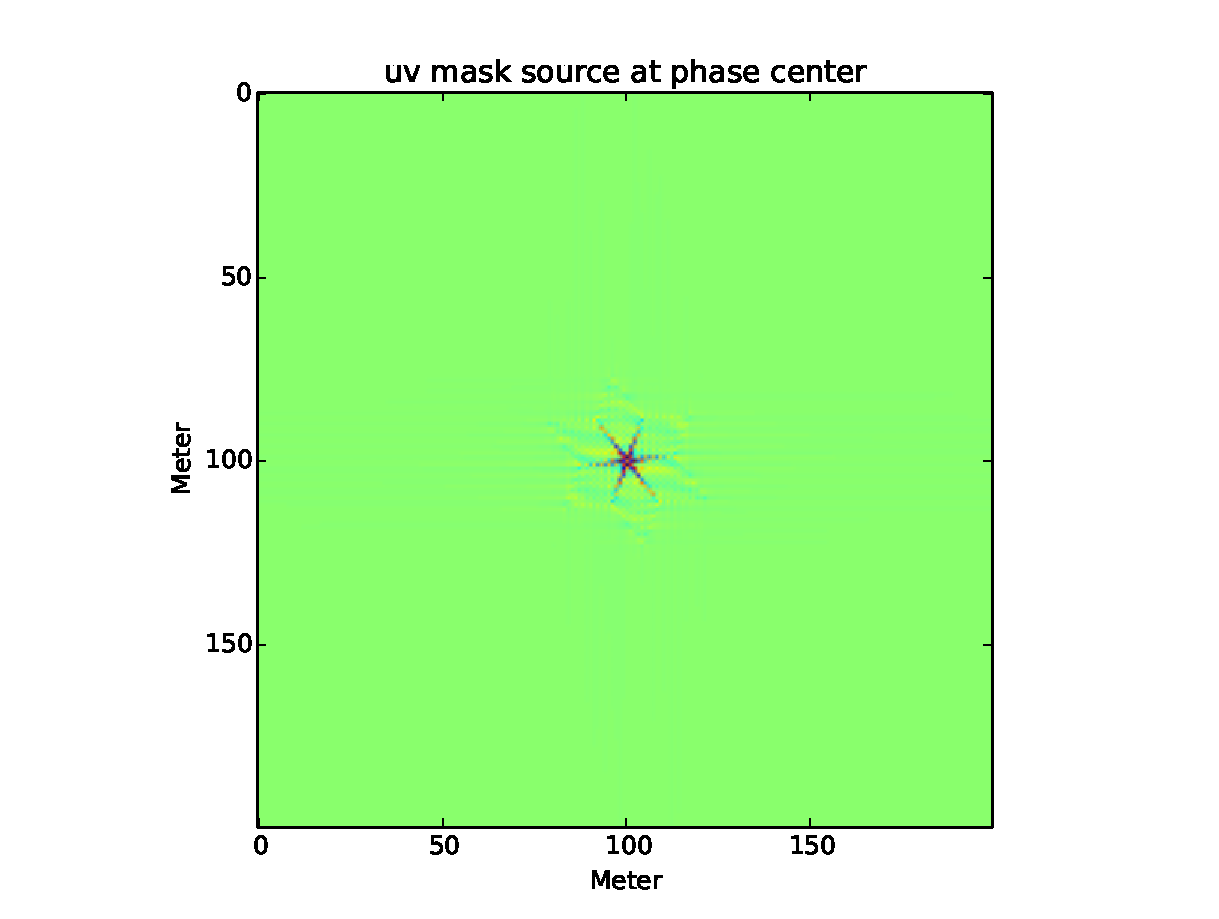
\includegraphics[width=.5\textwidth]{./Figures/uv.pdf}%
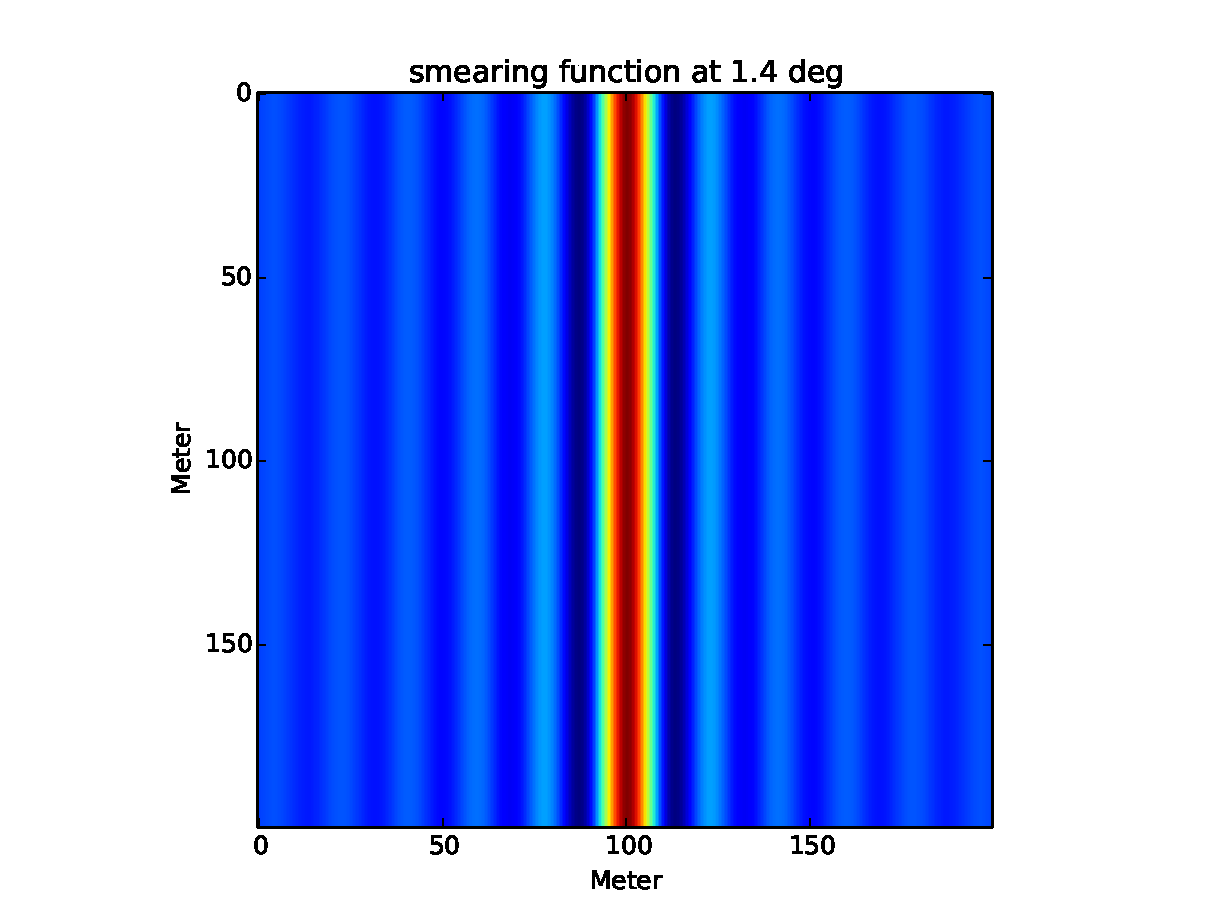
\includegraphics[width=.5\textwidth]{./Figures/smearing_uv.pdf}
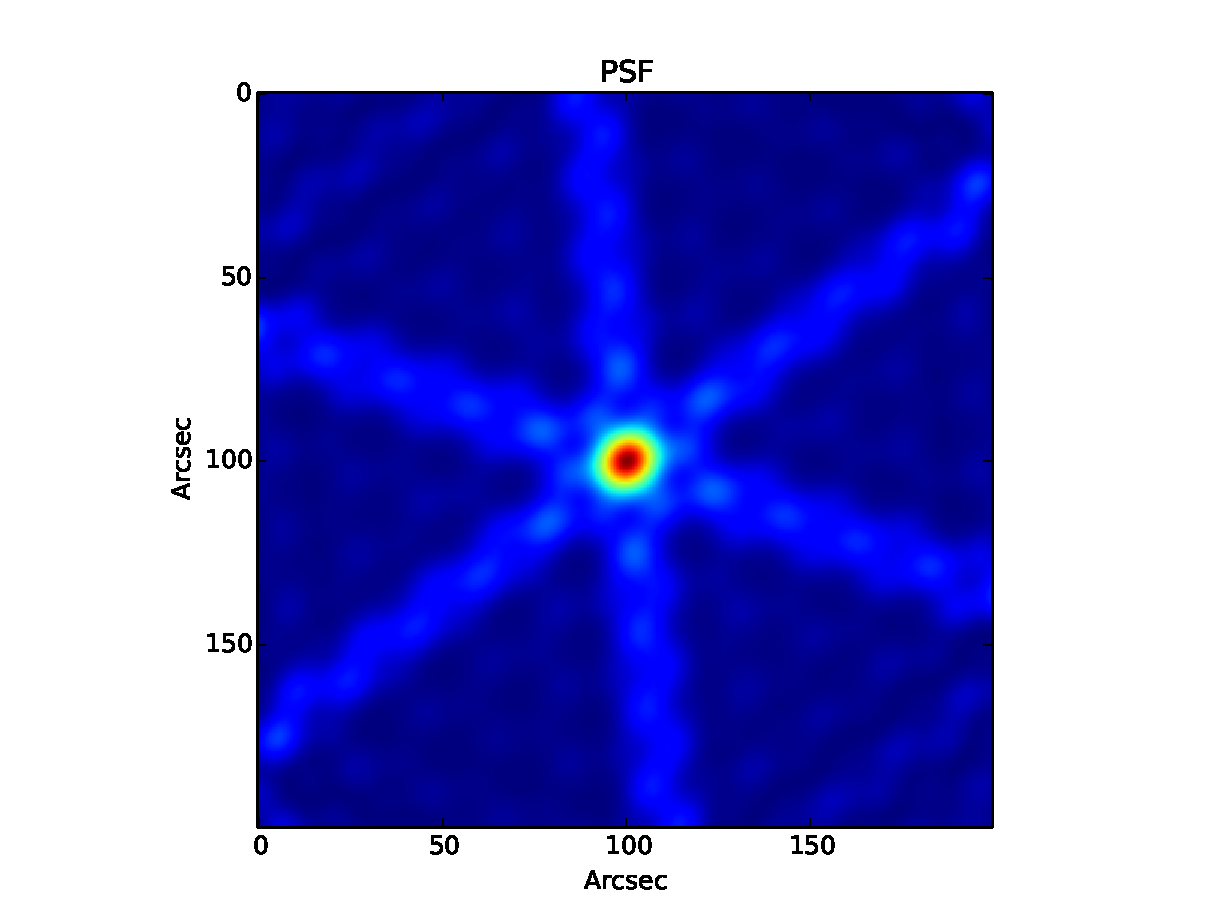
\includegraphics[width=.5\textwidth]{./Figures/psf.pdf}%
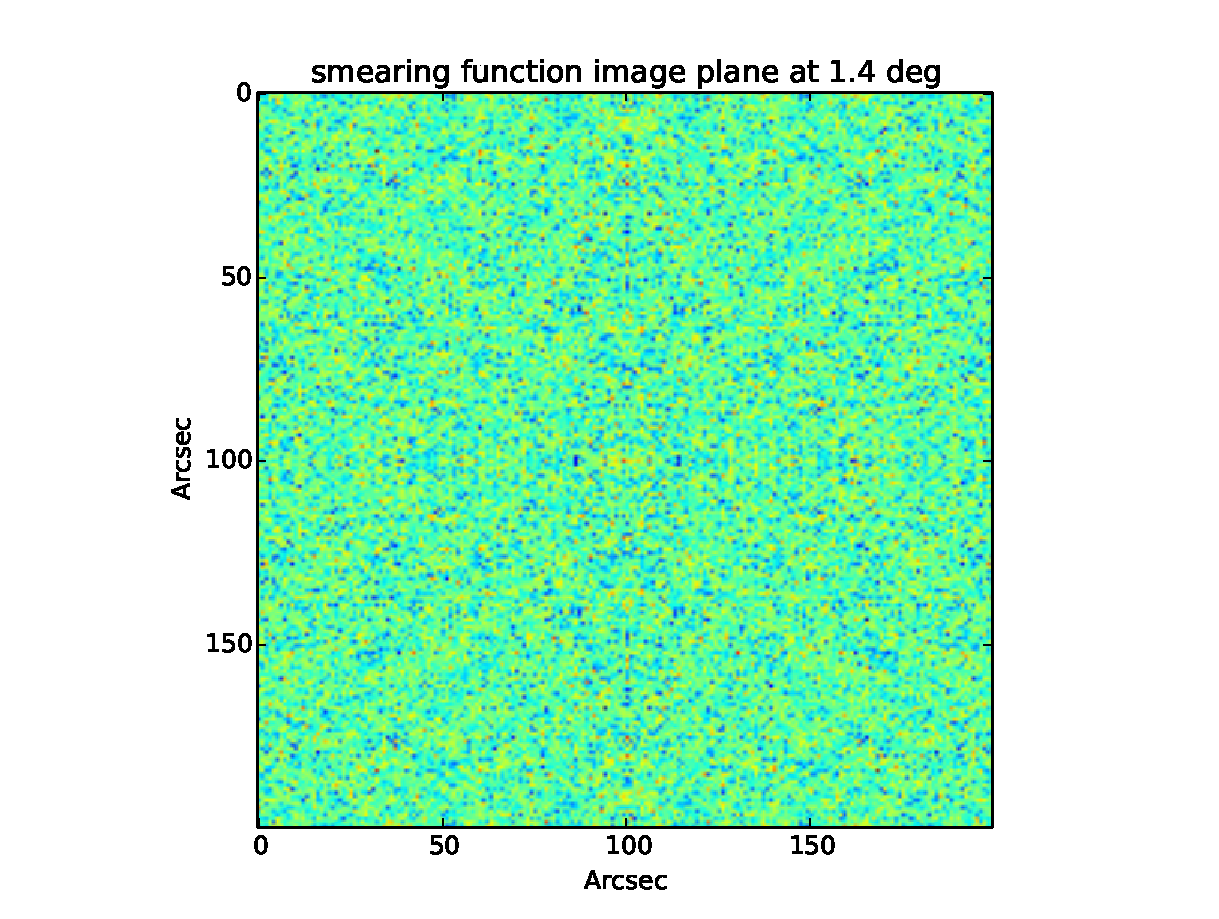
\includegraphics[width=.5\textwidth]{./Figures/smearing_imagePlane.pdf}
\caption{Hanning-Bessel windowing function and its tapering response.}\label{fig:wf:bessel-han}
\end{figure*}
\begin{figure*}
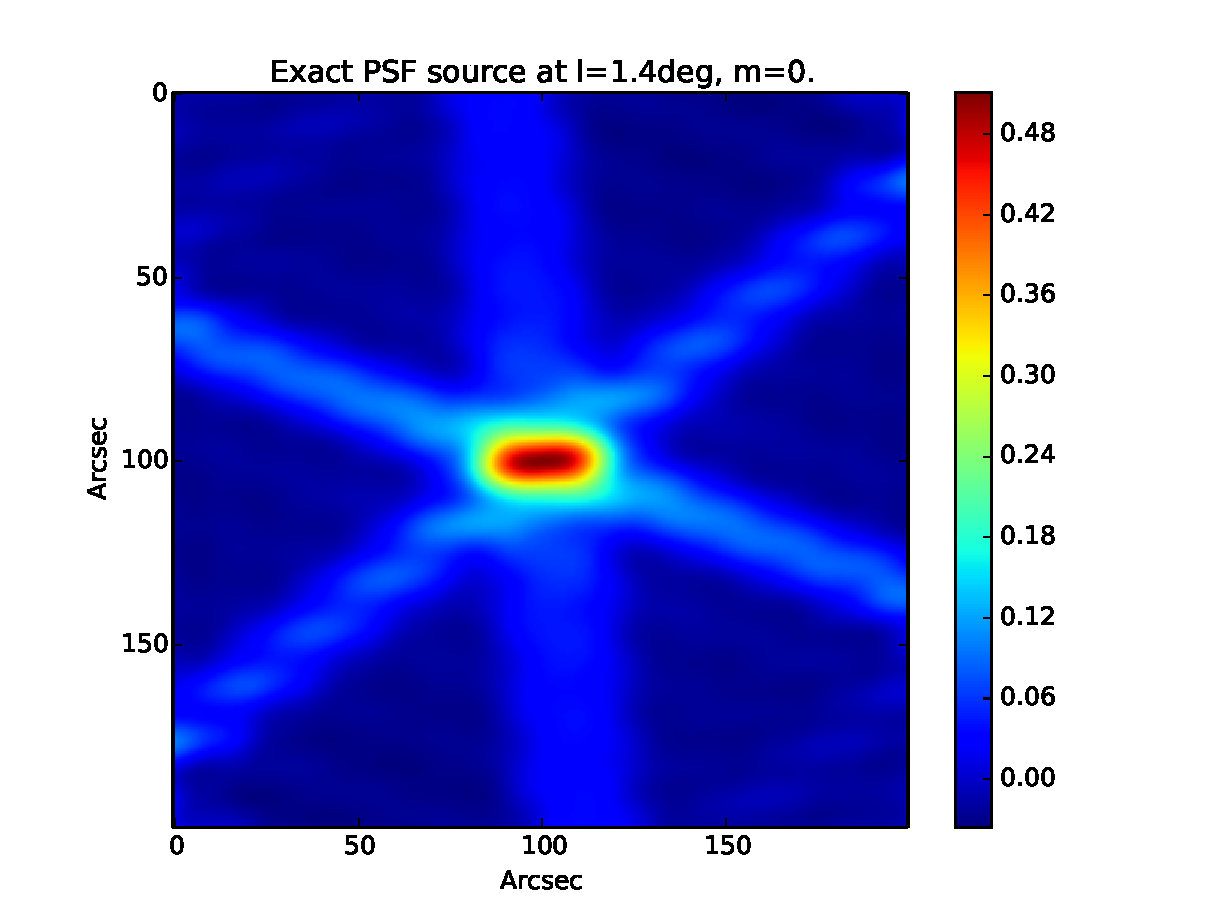
\includegraphics[width=.5\textwidth]{./Figures/exact_14deg.pdf}%
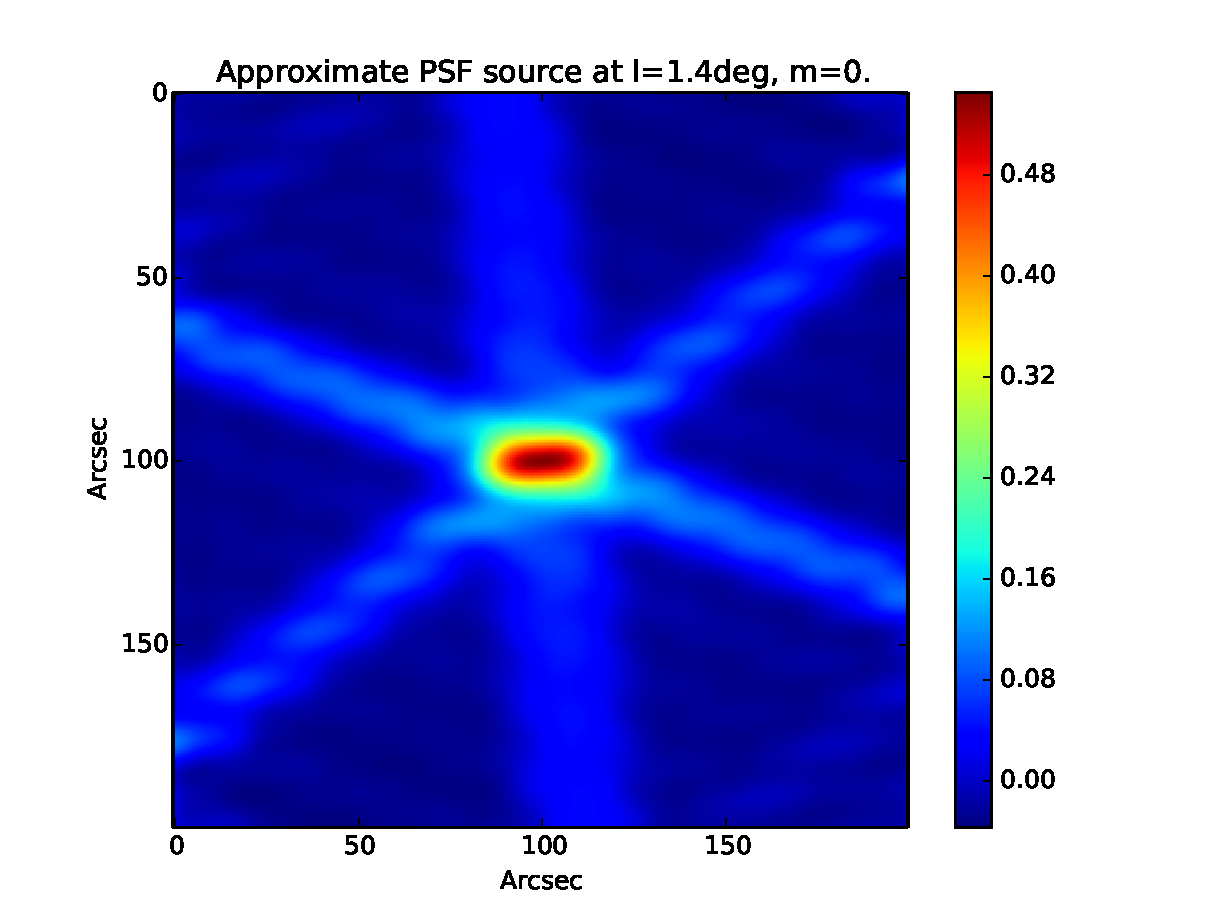
\includegraphics[width=.5\textwidth]{./Figures/approximate.pdf}
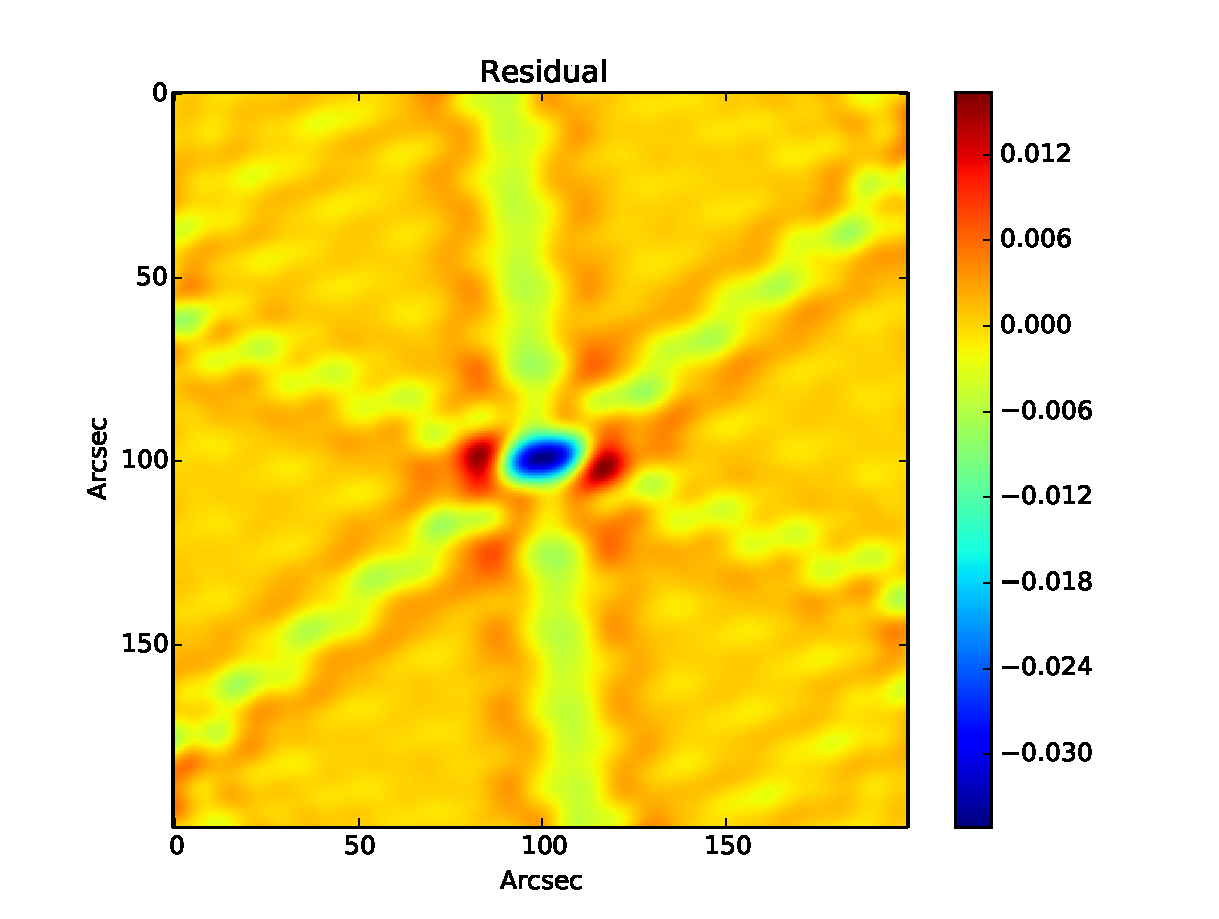
\includegraphics[width=.5\textwidth]{./Figures/residual_14deg.pdf}%
\caption{Hanning-Bessel windowing function and its tapering response.}\label{fig:wf:bessel-han}
\end{figure*}

 \section{DISCUSSION AND CONCLUSION}
 

